\documentclass[12pt, twoside]{article}
\usepackage[letterpaper, margin=1in, headsep=0.5in]{geometry}
\usepackage[english]{babel}
\usepackage[utf8]{inputenc}
\usepackage{amsmath}
\usepackage{amsfonts}
\usepackage{amssymb}
\usepackage{tikz}
%\usetikzlibrary{quotes, angles}

\usepackage{graphicx}
\usepackage{enumitem}
\usepackage{multicol}

\usepackage{fancyhdr}
\pagestyle{fancy}
\fancyhf{}
\renewcommand{\headrulewidth}{0pt} % disable the underline of the header

\fancyhead[RE]{\thepage}
\fancyhead[RO]{\thepage \\ Name: \hspace{3cm}}
\fancyhead[L]{BECA / Dr. Huson / 10th Grade Geometry\\* 21 March 2019}

\begin{document}
\subsubsection*{8-13 Unit Test: Similar triangles, dilation ratios, transformations}
 \begin{enumerate}

  \begin{multicols}{2}
  [\item A dilation maps triangle $PQR$ onto triangle $STU$ with $QR=7$ and $TU=14$.] \vspace{0.75cm}
    \begin{enumerate}
      \item $\overline{PR} \rightarrow$ \rule{2cm}{0.15mm}
      \item What scale factor maps\\
       $\triangle PQR \rightarrow \triangle STU$? \vspace{0.75cm}
      \item Given $PR=10$, find $SU$. \vspace{0.75cm}
      \item Given $ST=6$, find $PQ$.
      \end{enumerate}
      \begin{tikzpicture}[scale=0.9]
        \coordinate [label=above left:$P$](A) at (85:2);
        \coordinate [label=below:$Q$](B) at (0, 0);
        \coordinate [label=right:$R$](C) at (-20:3);
        \draw [thick] (A)--(B)--(C)--cycle;
        \draw [thick, xshift=2cm, yshift=2.5cm] (85:3) node[above]{$S$}--
        (0,0) node[below]{$T$}--
        (-20:4.5) node[right]{$U$}--cycle;
      \end{tikzpicture}
    \end{multicols}  \vspace{1cm}

  \item After a dilation with center $(0,0)$, the image of $\overline{MN}$ is $\overline{M'N'}$. If $MN=7.2$ and $M'N'=36$, find the scale factor of this dilation. \vspace{3cm}


  \item In the diagram below, $\triangle ABC$ with sides of 10, 12, and 11, is mapped onto $\triangle DEF$ after a clockwise rotation of $90^\circ$ about point $P$.
      \begin{center}
        \begin{tikzpicture}[scale=.6]
        \fill (0,0) circle[radius=0.1] node[right]{$P$};
          \draw [thick]
          (-2,1) node[below left] {$A$}--
          (-7,2) node[left] {$B$}--
          (-4,5) node[above right] {$C$}--cycle;
            \node at (-5,1.5)[below]{10};
            \node at (-6,4){12};
            \node at (-2.5,3.5){11};
            \node at (6,5.5){$2x+4$};
          \draw [thick]
          (1,2) node[left] {$D$}--
          (2,7) node[above] {$E$}--
          (5,4) node[right] {$F$}--cycle;
        \end{tikzpicture}
      \end{center}
    If $EF=2x+4$, what is the value of $x$? \vspace{2cm}

\newpage
  \item The vertices of $\triangle JKL$ have the coordinates $J(-4,-2)$, $K(4,0)$, and $L(-2,4)$, as shown. \\[0.25cm]
    Apply a dilation to $\triangle JKL \rightarrow \triangle J'K'L'$, centered on the origin and with a scale factor $k=1.5$. Draw the image $\triangle J'K'L'$ on the set of axes below, labeling the vertices, and make a table showing the correspondence of both triangles' coordinate pairs.  \vspace{4cm}
    \begin{center}
      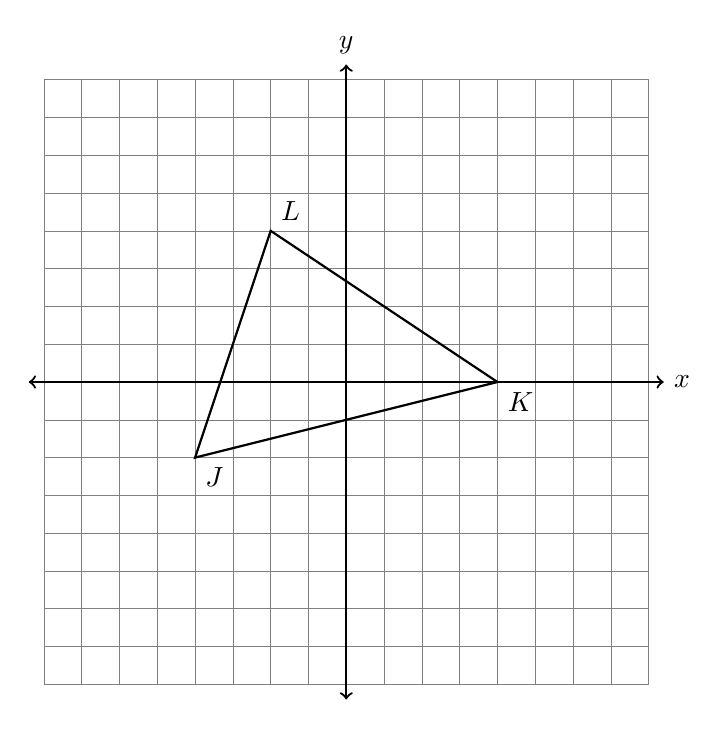
\begin{tikzpicture}[scale=.48]
        \draw [help lines] (-8,-8) grid (8,8);
        \draw [thick, <->] (-8.4,0) -- (8.4,0) node [right] {$x$};
        \draw [thick, <->] (0,-8.4)--(0,8.4) node [above] {$y$};
        \draw [thick]
        (-4,-2) node[below right] {$J$}--
        (4,0) node[below right] {$K$}--
        (-2,4) node[above right] {$L$}--
        cycle;
      \end{tikzpicture}
    \end{center}

\newpage
 \item Triangle $ABC$ is dilated with a scale factor of $k$ centered at $A$, yielding $\triangle ADE$, as shown. Given $AB=10$, $BC=14$, $AC=16$, and $DE=21$. \\[0.25cm] Find $BD$, $AE$, and $k$ (the scale factor). \vspace{0.5cm}
 \begin{center}
     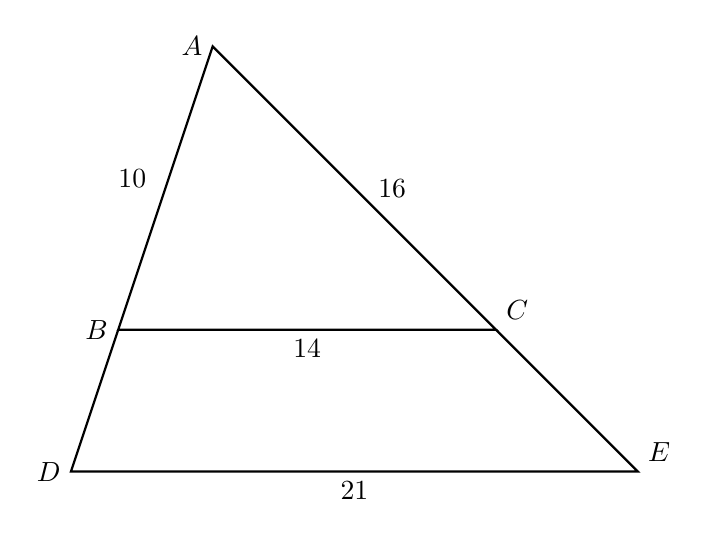
\begin{tikzpicture}[scale=0.6]
       \draw [thick]
       (0,0)node[left]{$B$}--
       (8,0)node[above right]{$C$}--
       (2,6)node[left]{$A$}--cycle;
       \draw [thick]
       (0,0)--
       (-1,-3)node[left]{$D$}--
       (11,-3)node[above right]{$E$}--(8,0);
       \node at (4,0)[below]{$14$};
       \node at (5.3, 3)[right]{$16$};
       \node at (0.3, 2.8)[above]{$10$};
       \node at (5,-3)[below]{$21$};
     \end{tikzpicture}
   \end{center}
\vspace{4cm}


 \begin{multicols}{2} [\item Circle YES or NO to indicate whether the given transformation maps the hexagon $ABCDEF$ onto itself.]
 \vspace{0.5cm}
  \begin{enumerate}
    \item Yes \quad No \quad A rotation of $120^\circ$ counterclockwise around point $D$.
     \item Yes \quad No \quad A reflection over $\overleftrightarrow{AE}$
     \item Yes \quad No \quad A reflection over a line through the midpoints of  $\overline{BC}$ and $\overline{EF}$.
     \item Yes \quad No \quad A rotation of $60^\circ$ clockwise around the hexagon's center.
     \end{enumerate}
   \begin{center}
       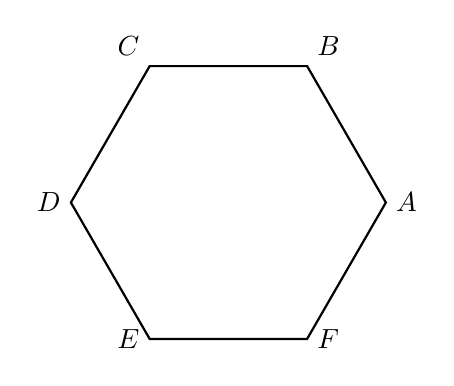
\begin{tikzpicture}%[scale=.48]
         \draw [thick]
         (0:2) node[right] {$A$}--
         (60:2) node[above right] {$B$}--
         (120:2) node[above left] {$C$} --
         (180:2) node[left] {$D$}--
         (240:2) node[left] {$E$}--
         (300:2) node[right] {$F$}--cycle;
       \end{tikzpicture}
     \end{center}
   \end{multicols} \vspace{0.5cm}

\newpage
   \item In right triangle $ABC$ shown below, point $D$ is on $\overline{AB}$ and point $E$ is on $\overline{BC}$ such that $\overline{AC} \parallel \overline{DE}$
     \begin{center}
       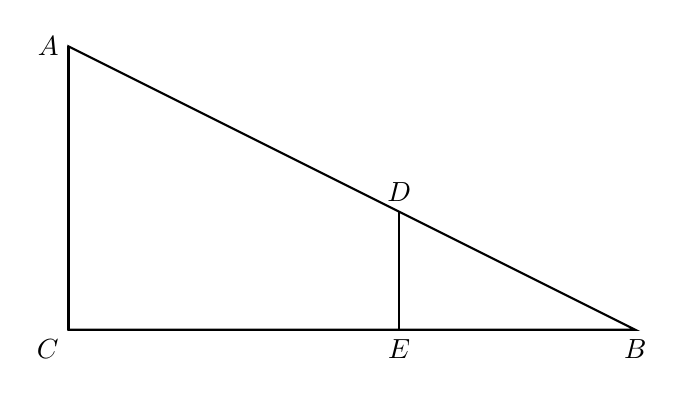
\begin{tikzpicture}[scale=0.6]
         \coordinate [label=left:$A$](A) at (-12,6);
         \coordinate [label=below:$B$](B) at (0, 0);
         \coordinate [label=below left:$C$](C) at (-12,0);
         \coordinate [label=above:$D$](D) at (-5, 2.5);
         \coordinate [label=below:$E$](E) at (-5,0);
         \draw [thick] (A)--(B)--(C)--cycle;
         \draw [thick] (A)--(C);
         \draw [thick] (D)--(E);
       \end{tikzpicture}
     \end{center}
   If $AB=20$, $BC=15$, and $AD=12$, what is the length of $\overline{BE}$?
   \vspace{3cm}

  \item What series of transformations map $\triangle ABC$ onto $\triangle DEF$, shown below? Fully specify the transformations.
    \begin{center}
      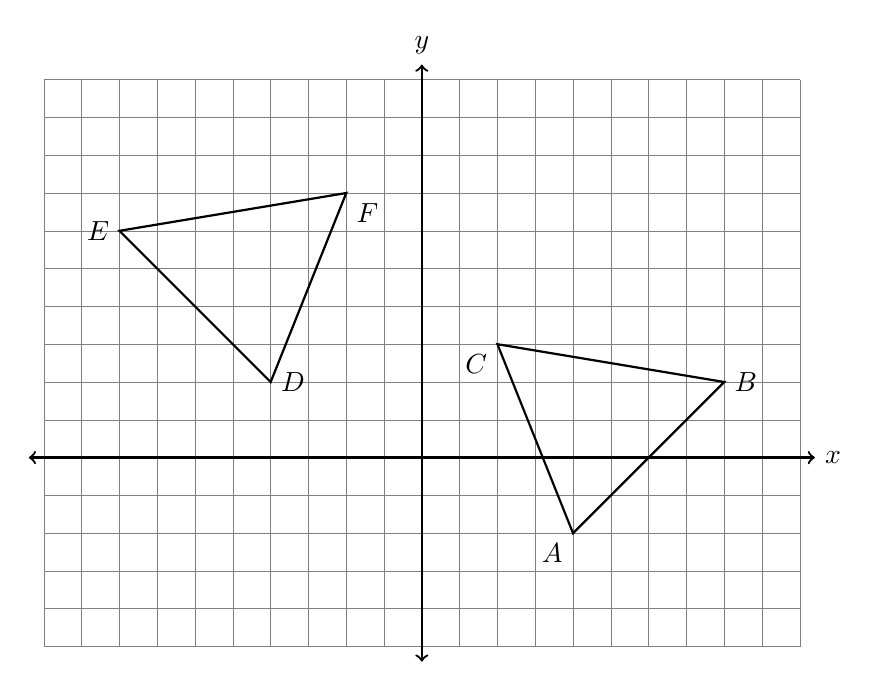
\begin{tikzpicture}[scale=.48]
        \draw [help lines] (-10,-5) grid (10,10);
        \draw [thick, <->] (-10.4,0) -- (10.4,0) node [right] {$x$};
        \draw [thick, <->] (0,-5.4)--(0,10.4) node [above] {$y$};
        \draw [thick]
          (4,-2) node[below left] {$A$}--
          (8,2) node[right] {$B$}--
          (2,3) node[below left] {$C$}--cycle;
        \draw [thick]
          (-4,2) node[right] {$D$}--
          (-8,6) node[left] {$E$}--
          (-2,7) node[below right] {$F$}--cycle;
      \end{tikzpicture}
    \end{center}
\vspace{2cm}

\newpage

  \item What is the length of the segment $A(-2,1)$, $B(3,13)$?
    \vspace{6cm}

  \item What is the equation of a line through the point $A(5,-1)$ and parallel to the line $y=\frac{2}{3}x-2$? (hint: use the point-slope formula, $y-y_A=m (x-x_A)$) \vspace{2.5cm}


  \item The line $l$ has the equation $y=-\frac{3}{5}x+4$. To each line below, circle whether $l$ is parallel, perpendicular, or neither.
    \begin{enumerate}
      \item parallel \quad perpendicular \quad neither \qquad $y=\frac{3}{5}x-2$
      \vspace{0.5cm}
      \item parallel \quad perpendicular \quad neither \qquad $y=\frac{5}{3}x+9$
      \vspace{0.5cm}
      \item parallel \quad perpendicular \quad neither \qquad $3x-5y=-15$
      \vspace{2cm}
      \item parallel \quad perpendicular \quad neither \qquad $5x-3y=6$
      \vspace{1.7cm}
    \end{enumerate}

  \item Simplify each expression. (Leave it in radical form if necessary, not a decimal.)
    \begin{enumerate}
      \begin{multicols}{2}
      \item   $\sqrt{20}$ \vspace{1.25cm}
      \item   $\sqrt{75}$
      \item   $\sqrt{300}$ \vspace{1.25cm}
      \item   $\sqrt{\frac{36}{49}}$
      \end{multicols}
    \end{enumerate}

\newpage

 \item Given $\triangle ABP$ and $\triangle JKP$ as shown below. $\overline{AB} \parallel \overline{JK}$. $AP=5$, $JP=12$, and $JK=18$. Find $AB$.
 \begin{center}
   \begin{tikzpicture}[scale=1.4]
       \draw [thick]
         (0.25,-1)node[right]{$B$}--
         (-0.5,2)node[left]{$K$}--
         (4,0)node[right]{$J$}--
         (0,0)node[above right]{$P$}--
         (-2,0)node[left]{$A$}--cycle;
     \end{tikzpicture}
     \end{center}
 \vspace{2cm}

\item The $\triangle ABC$ is reflected across $l$ to yield $\triangle A'B'C'$. $AB=3x+4$, $A'B'=5x-10$, and $BC=4x+12$. Find the length $B'C'$. %\vspace{2cm}
    \begin{center}
    \begin{tikzpicture}[scale=.8]
      \draw [dashed, <->] (-1,-1)--(7,7) node[below right]{$l$};
      \draw [thick]
      (5,-1) node[below right] {$A$}--
      (8,2) node[right] {$B$}--
      (1,0) node[below left] {$C$}--cycle;
      \draw [thick]
      (-1,5) node[left] {$A'$}--
      (2,8) node[below right] {$B'$}--
      (0,1) node[below left] {$C'$}--cycle;
    \end{tikzpicture}
  \end{center} \vspace{2cm}

\newpage
 \item The figure shows a rectangle (not a square).
   \begin{center}
     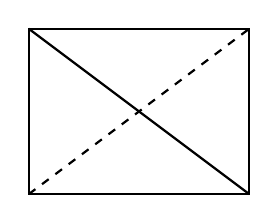
\begin{tikzpicture}[scale=0.7]
       \coordinate (A) at (0, 0); %[label=above left:$P$]
       \coordinate (B) at (4, 0);
       \coordinate (C) at (4, 3);
       \coordinate (D) at (0, 3);
       \draw [thick] (A)--(B)--(C)--(D)--cycle;
       \draw [thick, dashed] (A)--(C);
       \draw [thick] (B)--(D);
       %\draw [thick, xshift=2cm, yshift=2.5cm] (85:3);
     \end{tikzpicture}
   \end{center}
   Which transformations carries the rectangle onto itself? Mark each True or False.
     \begin{enumerate}
       \item A reflection over the solid diagonal \hfill True \quad False
       \item A reflection over the dashed diagonal \hfill True \quad False
       \item A clockwise rotation of $90^\circ$ about the intersection of the diagonals \hfill True \quad False
       \item A clockwise rotation of $180^\circ$ about the intersection of the diagonals \hfill True \quad False
     \end{enumerate}
     \vspace{1cm}

   \item The grid shows $\triangle ABC$ and $\triangle DEF$.
     \begin{center}
       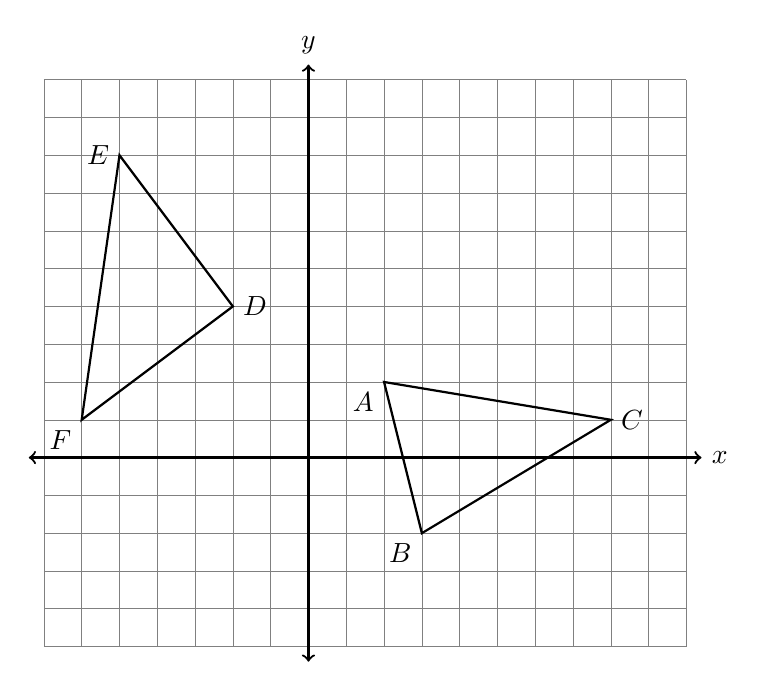
\begin{tikzpicture}[scale=.48]
         \draw [help lines] (-7,-5) grid (10,10);
         \draw [thick, <->] (-7.4,0) -- (10.4,0) node [right] {$x$};
         \draw [thick, <->] (0,-5.4)--(0,10.4) node [above] {$y$};
         \draw [thick]
           (3,-2) node[below left] {$B$}--
           (8,1) node[right] {$C$}--
           (2,2) node[below left] {$A$}--cycle;
         \draw [thick]
           (-2,4) node[right] {$D$}--
           (-5,8) node[left] {$E$}--
           (-6,1) node[below left] {$F$}--cycle;
       \end{tikzpicture}
     \end{center}
     Let $\triangle A'B'C'$ be the image of $\triangle ABC$ after a rotation about point $A$. Determine and state the location of $B'$ if the location of point $C'$ is $(3,8)$. Explain your answer, supported by stating the transformation applied.

 \newpage

   \item What is the smallest non-zero angle of rotation about its center that would map pentagon $ABCDE$ onto itself? \vspace{0.25cm}
   \begin{center}
       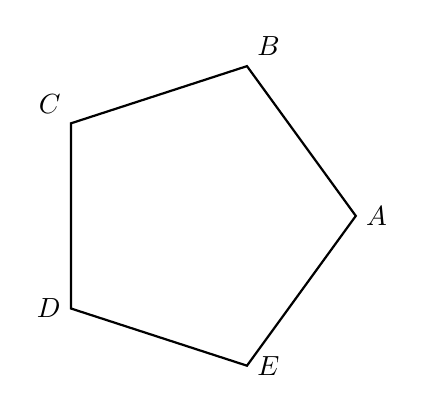
\begin{tikzpicture}%[scale=.48]
         \draw [thick]
         (0:2) node[right] {$A$}--
         (72:2) node[above right] {$B$}--
         (144:2) node[above left] {$C$} --
         (216:2) node[left] {$D$}--
         (288:2) node[right] {$E$}--cycle;
       \end{tikzpicture}
     \end{center} \vspace{0.5cm}

  \item Triangle $ADE$ and its midline $\overline{BC}$ are drawn, with $B$ the midpoint of $\overline{AD}$ and $C$ the midpoint of $\overline{AE}$. The two medians $\overline{BE}$ and $\overline{CD}$ are drawn, as shown, intersecting in point $F$, the centroid.\\[0.25cm]
  $\triangle FCB \sim \triangle FDE$ with scale factor $k=2$.\\[0.25cm]
  Given $BC=9$, find $DE$. \\[0.25cm] Given $FE=12$, find $BF$. %\vspace{1cm}
  \begin{center}
      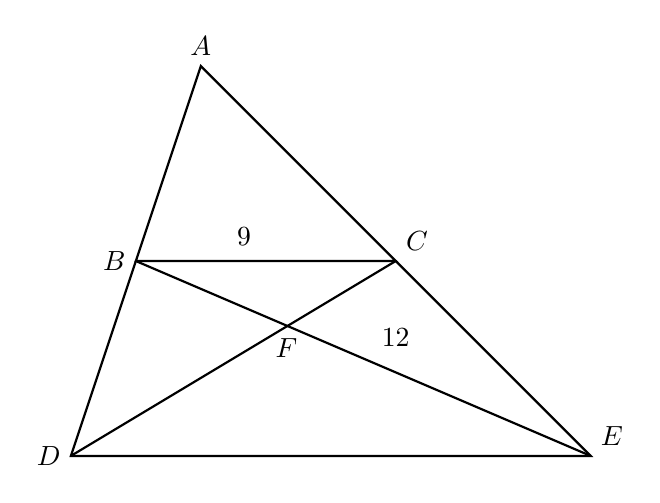
\begin{tikzpicture}[scale=0.55]
        \draw [thick]
        (0.5,1.5)node[left]{$B$}--
        (6.5,1.5)node[above right]{$C$}--
        (2,6)node[above]{$A$}--cycle;
        \draw [thick]
        (0.5,1.5)--
        (-1,-3)node[left]{$D$}--
        (11,-3)node[above right]{$E$}--(6.5,1.5);
        \draw [thick] (0.5,1.5)--(11,-3);
        \draw [thick] (6.5,1.5)--(-1,-3);
        \node at (3,2.5)[below]{$9$};
        \node at (3.5, -0.5)[right]{$F$};
        \node at (6.5, -.7)[above]{$12$};
        %\node at (-0.7, -1)[above]{$5$};
      \end{tikzpicture}
    \end{center} \vspace{1cm}

  \item Write down the center and radius of each circle.
    \begin{enumerate}
      \begin{multicols}{2}
      \item   $(x+1)^2+(y-1)^2=16$ \vspace{2cm}
      \item   $(x-2)^2+(y-7)^2=25$ \vspace{2cm}
      \end{multicols}
    \end{enumerate}

\newpage
 \item Determine and state the transformation or sequence of transformations  applied to $\triangle ABC$, mapping it onto $\triangle PQR$, as shown.
   \begin{center}
       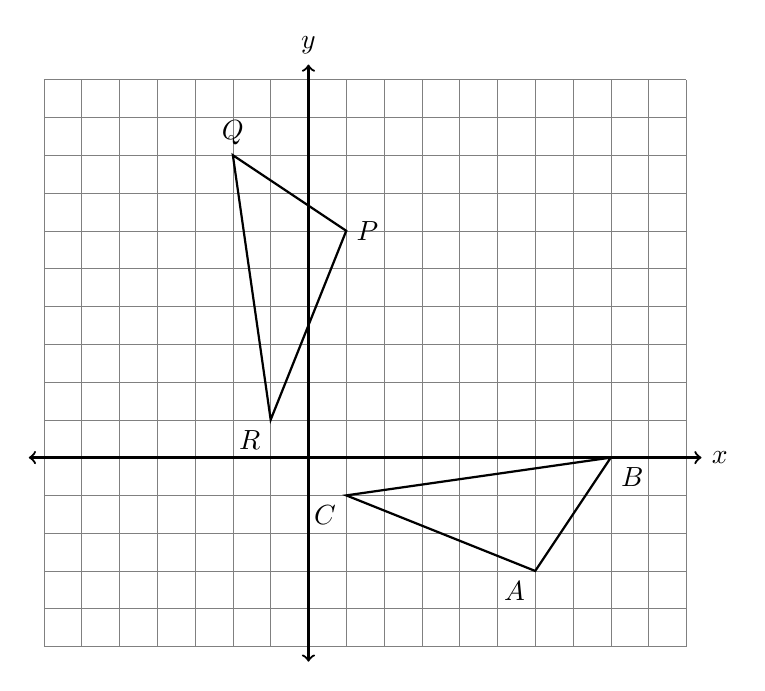
\begin{tikzpicture}[scale=.48]
         \draw [help lines] (-7,-5) grid (10,10);
         \draw [thick, <->] (-7.4,0) -- (10.4,0) node [right] {$x$};
         \draw [thick, <->] (0,-5.4)--(0,10.4) node [above] {$y$};

         \draw [thick]
         (6,-3) node[below left] {$A$}--
         (8,0) node[below right] {$B$}--
         (1,-1) node[below left] {$C$}--cycle;

         \draw [thick]
         (1,6) node[right] {$P$}--
         (-2,8) node[above] {$Q$}--
         (-1,1) node[below left] {$R$}--cycle;
       \end{tikzpicture}
     \end{center}
\vspace{2cm}

  \begin{multicols}{2}[\item The diagram below shows $\triangle ABC$, with $\overline{AEB}$, $\overline{ADC}$, and $\angle ACB \cong \angle AED$. $AB=14$, $AD=8$, and $DE=4$.]
      \begin{enumerate}
        \item $\overline{AE} \rightarrow$ \rule{2cm}{0.15mm} \vspace{0.5cm}
        \item $\overline{AD} \rightarrow$ \rule{2cm}{0.15mm} \vspace{0.5cm}
        \item $\triangle ADE \sim$ \rule{2cm}{0.15mm} \vspace{0.5cm}
        \item What is the scale factor?\\[0.5cm] $k=$  \rule{2cm}{0.15mm}
        \item What is the length of $\overline{BC}$?
      \end{enumerate}
       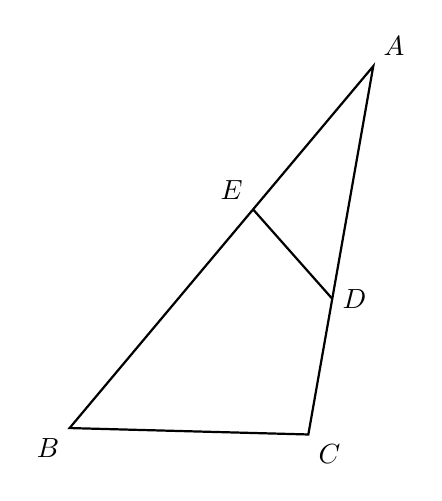
\begin{tikzpicture}%[scale=.48]
         \draw [thick]
         (0,0) node[above right] {$A$}--
         (230:6) node[below left] {$B$}--
         (260:4.75) node[below right] {$C$}--cycle;
         \draw [thick]
         (230:2.375) node[above left] {$E$}--
         (260:3) node[right] {$D$}--cycle;
       \end{tikzpicture}
     \end{multicols}

\newpage


  \item Given $\triangle JKL \sim \triangle MNO$. $m\angle J = 43^\circ$ and $m\angle L = 92^\circ$.\\
  Find the measure of $\angle N$. \vspace{1.5cm}

  \item A translation maps $A(3,5) \rightarrow A'(-2,7)$. What is the image of $B(-4,1)$ under the same translation?  \vspace{1.5cm}


  \item As shown below, what is the translation that maps the point $R(-4,4)$ onto the point $S(6, -1)$?
    \begin{center} %4 quadrant regents grid
      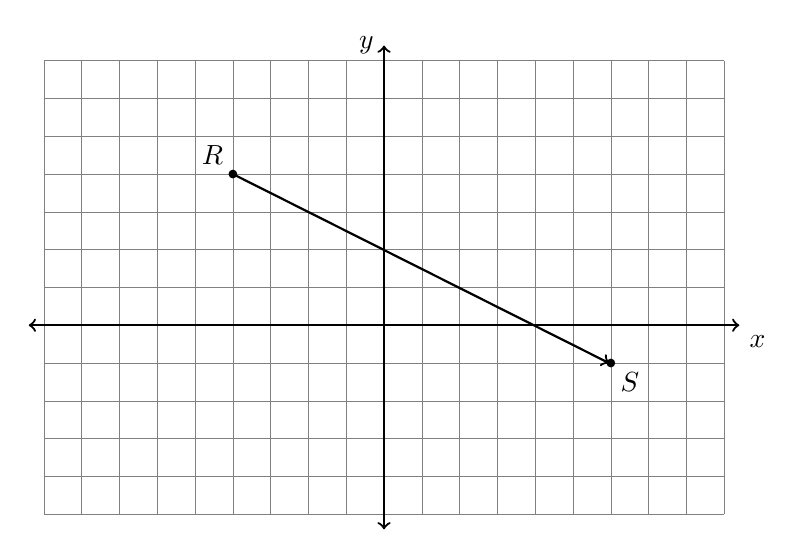
\begin{tikzpicture}[scale=.48]
        \draw [help lines] (-9,-5) grid (9,7);
        \draw [thick, <->] (-9.4,0) -- (9.4,0) node [below right] {$x$};
        \draw [thick, <->] (0,-5.4)--(0,7.4) node [left] {$y$};
        \draw [thick, ->] (-4,4)--(5.95, -1);
        \draw [fill] (-4,4) circle [radius=0.1] node[above left] {$R$};
        \draw [fill] (6, -1) circle [radius=0.1] node[below right] {$S$};
      \end{tikzpicture}
    \end{center}
    If two fifths of that translation was performed, what coordinates would $R$ be mapped to? \vspace{2.5cm}

  \item Given $A(-3,5)$ and $B(0,-1)$, find the length of $\overline{AB}$. Leave the result in simplified radical form (not a decimal).

\newpage
\emph{Early finishers}
  \item In the diagram below, the chords $\overline{AE}$ and $\overline{BD}$ intersect at $C$, with $\triangle ABC \sim \triangle DEC$, $BC=3$, $AC=4$, and $AE=11$. Determine the length of $\overline{CD}$.
      \begin{center}
      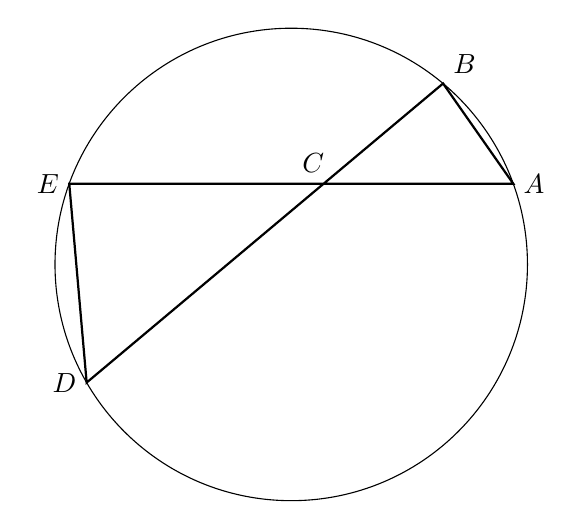
\begin{tikzpicture}[scale=.6]
        \draw (0,0) circle[radius=5];
        \draw [thick]
        (20:5) node[right] {$A$}--
        (160:5) node[left] {$E$}--
        (210:5) node[left] {$D$}--
        (50:5) node[above right] {$B$}--cycle;
        \draw (75:1.8) node[above] {$C$};
      \end{tikzpicture}
    \end{center}

\vspace{2cm}

  \item In the diagram below, $\triangle ABC \sim \triangle DEF$, $DE=6$, $AB=x$, $AC=2x$, and $DF=2x+4$. Determine the length of $\overline{AB}$.
    \begin{center}
      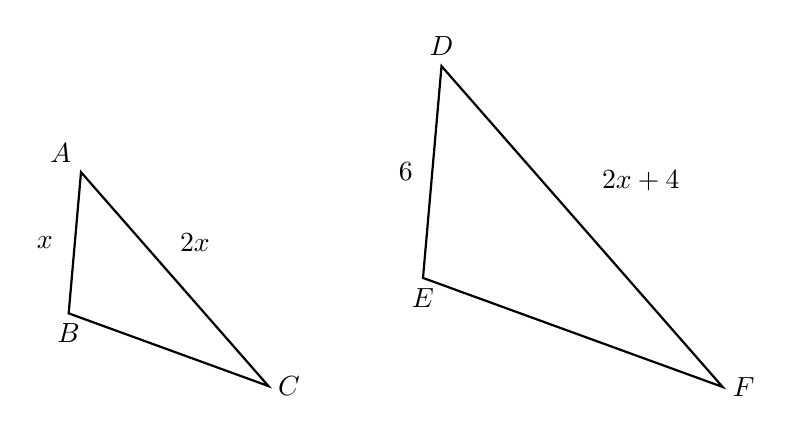
\begin{tikzpicture}[scale=0.9]
      \coordinate [label=above left:$A$](A) at (85:2);
      \coordinate [label=below:$B$](B) at (0, 0);
      \coordinate [label=right:$C$](C) at (-20:3);
        \draw [thick] (A)--(B)--(C)--cycle;
        \node at (95:1)[left]{$x$};
        \node at (35:1.75)[right]{$2x$};
        \draw [thick, xshift=5cm, yshift=0.5cm] (85:3) node[above]{$D$}--
        (0,0) node[below]{$E$}--
        (-20:4.5) node[right]{$F$}--cycle;
        \draw [thick, xshift=5cm, yshift=0.5cm](90:1.5) node[left]{$6$};
        \draw [thick, xshift=5cm, yshift=0.5cm](30:2.75) node[right]{$2x+4$};
    \end{tikzpicture}
    \end{center}


\end{enumerate}
\end{document}
